% Capítulo 7: busca sequencial do 42 em um vetor fora de ordem (5 comparações).
\documentclass[border=4pt]{standalone}
\usepackage[utf8]{inputenc}
\usepackage[T1]{fontenc}
% Estilo comum das figuras de listas (incluído pelas figuras dos capítulos 3 e 4).
\usepackage{tikz}
\usetikzlibrary{arrows.meta, positioning, shapes.multipart, calc}
\definecolor{navy}{RGB}{23,45,80}
\definecolor{laranja}{RGB}{250,110,29}
\definecolor{cinzalogo}{RGB}{107,114,126}
\tikzset{
  no/.style={rectangle split, rectangle split horizontal, rectangle split parts=2,
             draw=navy, line width=0.9pt, minimum height=7mm,
             rectangle split part fill={laranja!15, white}, font=\sffamily\small},
  no3/.style={rectangle split, rectangle split horizontal, rectangle split parts=3,
              draw=navy, line width=0.9pt, minimum height=7mm,
              rectangle split part fill={white, laranja!15, white}, font=\sffamily\small},
  seta/.style={-{Stealth[length=2.2mm]}, navy, line width=0.9pt},
  setanova/.style={-{Stealth[length=2.2mm]}, laranja, line width=1.3pt},
  rotulo/.style={font=\sffamily\small\bfseries, text=navy},
  nulo/.style={font=\sffamily\scriptsize, text=cinzalogo},
  passo/.style={font=\sffamily\small, text=cinzalogo, anchor=west},
  legenda/.style={font=\sffamily\scriptsize, text=cinzalogo},
}
% seta que sai do meio da caixa do ponteiro (última parte do nó), na horizontal
\newcommand{\liga}[3][seta]{\draw[#1] ([xshift=-2.3mm]#2.east) -- #3;}

\tikzset{
  casa/.style={draw=navy, line width=0.9pt, minimum width=10mm, minimum height=8mm, font=\sffamily\small},
  vista/.style={casa, fill=cinzalogo!20, text=cinzalogo},
  achou/.style={casa, fill=laranja!45, draw=laranja},
  indice/.style={font=\sffamily\scriptsize, text=cinzalogo},
}
\begin{document}
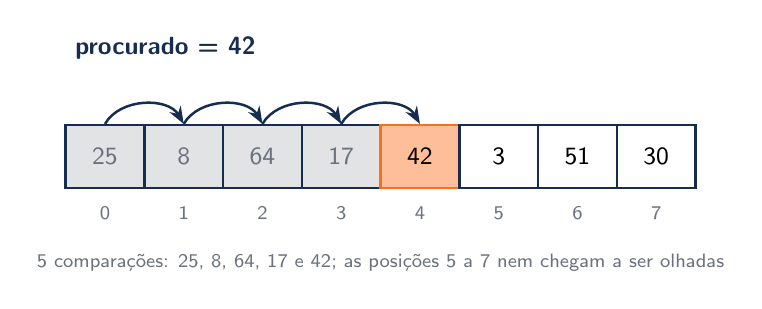
\begin{tikzpicture}
  \foreach \x [count=\i from 0] in {25, 8, 64, 17, 42, 3, 51, 30} {
    \ifnum\i<4
      \node[vista] (v\i) at (\i*1.0, 0) {\x};
    \else\ifnum\i=4
      \node[achou] (v\i) at (\i*1.0, 0) {\x};
    \else
      \node[casa] (v\i) at (\i*1.0, 0) {\x};
    \fi\fi
    \node[indice, below=1mm of v\i] {\i};
  }
  \foreach \i [evaluate=\i as \j using int(\i+1)] in {0,...,3} {
    \draw[seta] (v\i.north) to[out=60, in=120] (v\j.north);
  }
  \node[rotulo, above=7mm of v0, anchor=south west, xshift=-5mm] {procurado = 42};
  \node[legenda, below=7mm of v3, xshift=5mm]
    {5 comparações: 25, 8, 64, 17 e 42; as posições 5 a 7 nem chegam a ser olhadas};
\end{tikzpicture}
\end{document}
